\section{Open-World Environments}
\label{sec:open_world_environments}

Autonomous agents operate within environments that they must perceive, reason about, and act upon in order to achieve their goals. In this section, we formalize the structure of such environments and the agents that inhabit them, and distinguish between the closed-world settings that underlie most current AI research and the open-world settings that motivate this dissertation.

\subsection{The Environment}
\label{sec:environment}

We consider a task environment $\Env = \langle \EnvStates, \EnvDynamics \rangle$ consisting of a set of environment states $\EnvStates$ and a set of dynamics $\EnvDynamics$ that govern how states evolve over time. The environment may contain any number of objects and other agents as part of its state, and its dynamics may be deterministic or stochastic. Environment states are agent-independent in the sense that they specify the underlying configuration of the world whether or not any particular agent observes or represents them correctly.

At any given time $t$, the environment is in some state $e_t \in \EnvStates$. The dynamics $\EnvDynamics$ define how this state changes, both due to the natural evolution of the environment and as a consequence of actions taken by agents within it. In general, an agent does not have direct access to the full environment state $e_t$; instead, it observes the environment through its sensors and acts upon it through its effectors, as described below.

\subsection{The Agent}
\label{sec:agent}

An agent $\Agent = \langle \Sensors, \Effectors, \KnowledgeRepo, \vdash \rangle$ is defined by four components: a set of sensors $\Sensors$ that allow it to perceive the environment, a set of effectors $\Effectors$ that allow it to act upon it, a knowledge repository $\KnowledgeRepo$ that stores what the agent knows about the world, and an inference mechanism $\vdash$ that enables the agent to reason over its knowledge.

The knowledge repository $\KnowledgeRepo = (\KB, \SubsymbolicKB)$ is composed of two complementary parts. The knowledge base $\KB$ stores explicit symbolic knowledge---facts, rules, and relational descriptions expressed in a formal language $\Language$. The subsymbolic component $\SubsymbolicKB$ stores knowledge in distributed representations, such as the weights of neural networks that encode policies, value functions, or perceptual models. The inference mechanism $\vdash$ operates over both components: for $\KB$, it may take the form of logical deduction or planning; for $\SubsymbolicKB$, it corresponds to forward inference through learned models.

At time $t$, the agent's sensors generate internal representations of the partially observed environment state. Based on these observations and its knowledge $\KnowledgeRepo$, the agent selects actions through its inference mechanism and executes them via its effectors, producing changes in the environment state. This perceive--reason--act cycle defines the agent's ongoing interaction with the world.

\subsection{Closed-World and Open-World Assumptions}
\label{sec:closed_open}

The distinction between closed-world and open-world settings concerns the relationship between the agent's knowledge and the environment.

Under closed-world assumptions, the agent's representational vocabulary and task model are treated as fixed and sufficient for the situations the agent may encounter. Specifically, the relevant objects, predicates, observations, actions, rewards, dynamics, and action effects are assumed to fall within the agent's predefined modeling framework. This assumption has been productive: it underlies classical planning \citep{fikes1971strips, mcdermott1998pddl}, standard reinforcement learning formulations \citep{sutton2018reinforcement}, and many supervised learning approaches to perception. Under these assumptions, the primary challenge is computational---finding good plans, learning effective policies, or achieving accurate classification within a fixed representational space.

In open-world environments, this assumption is violated. The environment may contain objects, dynamics, or relationships that the agent's models do not represent. New objects may appear that do not correspond to any known category. Actions may produce effects that differ from what the agent's models predict. Task structure may change in ways that invalidate previously successful strategies. Critically, these changes need not be adversarial or extreme: even routine variation in everyday environments can fall outside the scope of models designed under closed-world assumptions.

This gap between the agent's knowledge and the true state of the world is not merely a quantitative shortcoming that can be addressed by training on more data or enumerating more states. It is a qualitative property of the agent--environment relationship: the world may contain structure that is not derivable from, or even expressible within, the agent's current representational framework. This observation motivates the formal treatment of novelty developed in the next section.

\subsection{A Running Example: The Crafting Agent}
\label{sec:running_example}

To make the framework concrete, we introduce a running example that will be used throughout this chapter and the remainder of the dissertation. Consider an agent operating in a gridworld environment inspired by the crafting mechanics of Minecraft. The environment contains objects such as trees, crafting tables, ores, and storage containers. The agent can perform actions such as navigating to objects, breaking trees to obtain logs, crafting logs into planks and sticks, and assembling complex items using crafting recipes. The agent's task is to craft a target item---say, a pogostick---which requires collecting and combining resources in a specific sequence.

In this setting, the agent maintains symbolic knowledge of the objects in the environment, their properties, the available crafting recipes, and the operators it can use (e.g., \texttt{break\_tree}, \texttt{craft\_planks}, \texttt{craft\_pogostick}). Each operator is associated with an executor---a policy that carries out the corresponding action in the environment. The agent generates a plan (a sequence of operators) and executes it step by step. Under closed-world conditions, where the environment matches the agent's models, this process succeeds reliably.

Now suppose the environment changes while the agent is performing its task. A new entity---a supplier---appears and may affect the agent's ability to obtain resources. Or the properties of a known object change: trees become unbreakable unless the agent first acquires a new tool, an axe. Or a crafting recipe is altered so that a previously unnecessary ingredient is now required. Each of these changes may constitute a novelty for the agent: an aspect of the environment that is not derivable from, or not expressible within, its current knowledge repository. How the agent responds---whether it can detect the change, diagnose its impact, and adapt its behavior---depends on the structure of its representations and reasoning capabilities. The formal treatment of novelty in \cref{sec:novelty} and the agent framework in \cref{sec:agent_framework} provide the machinery for analyzing these situations precisely.

\begin{figure}[t]
\centering
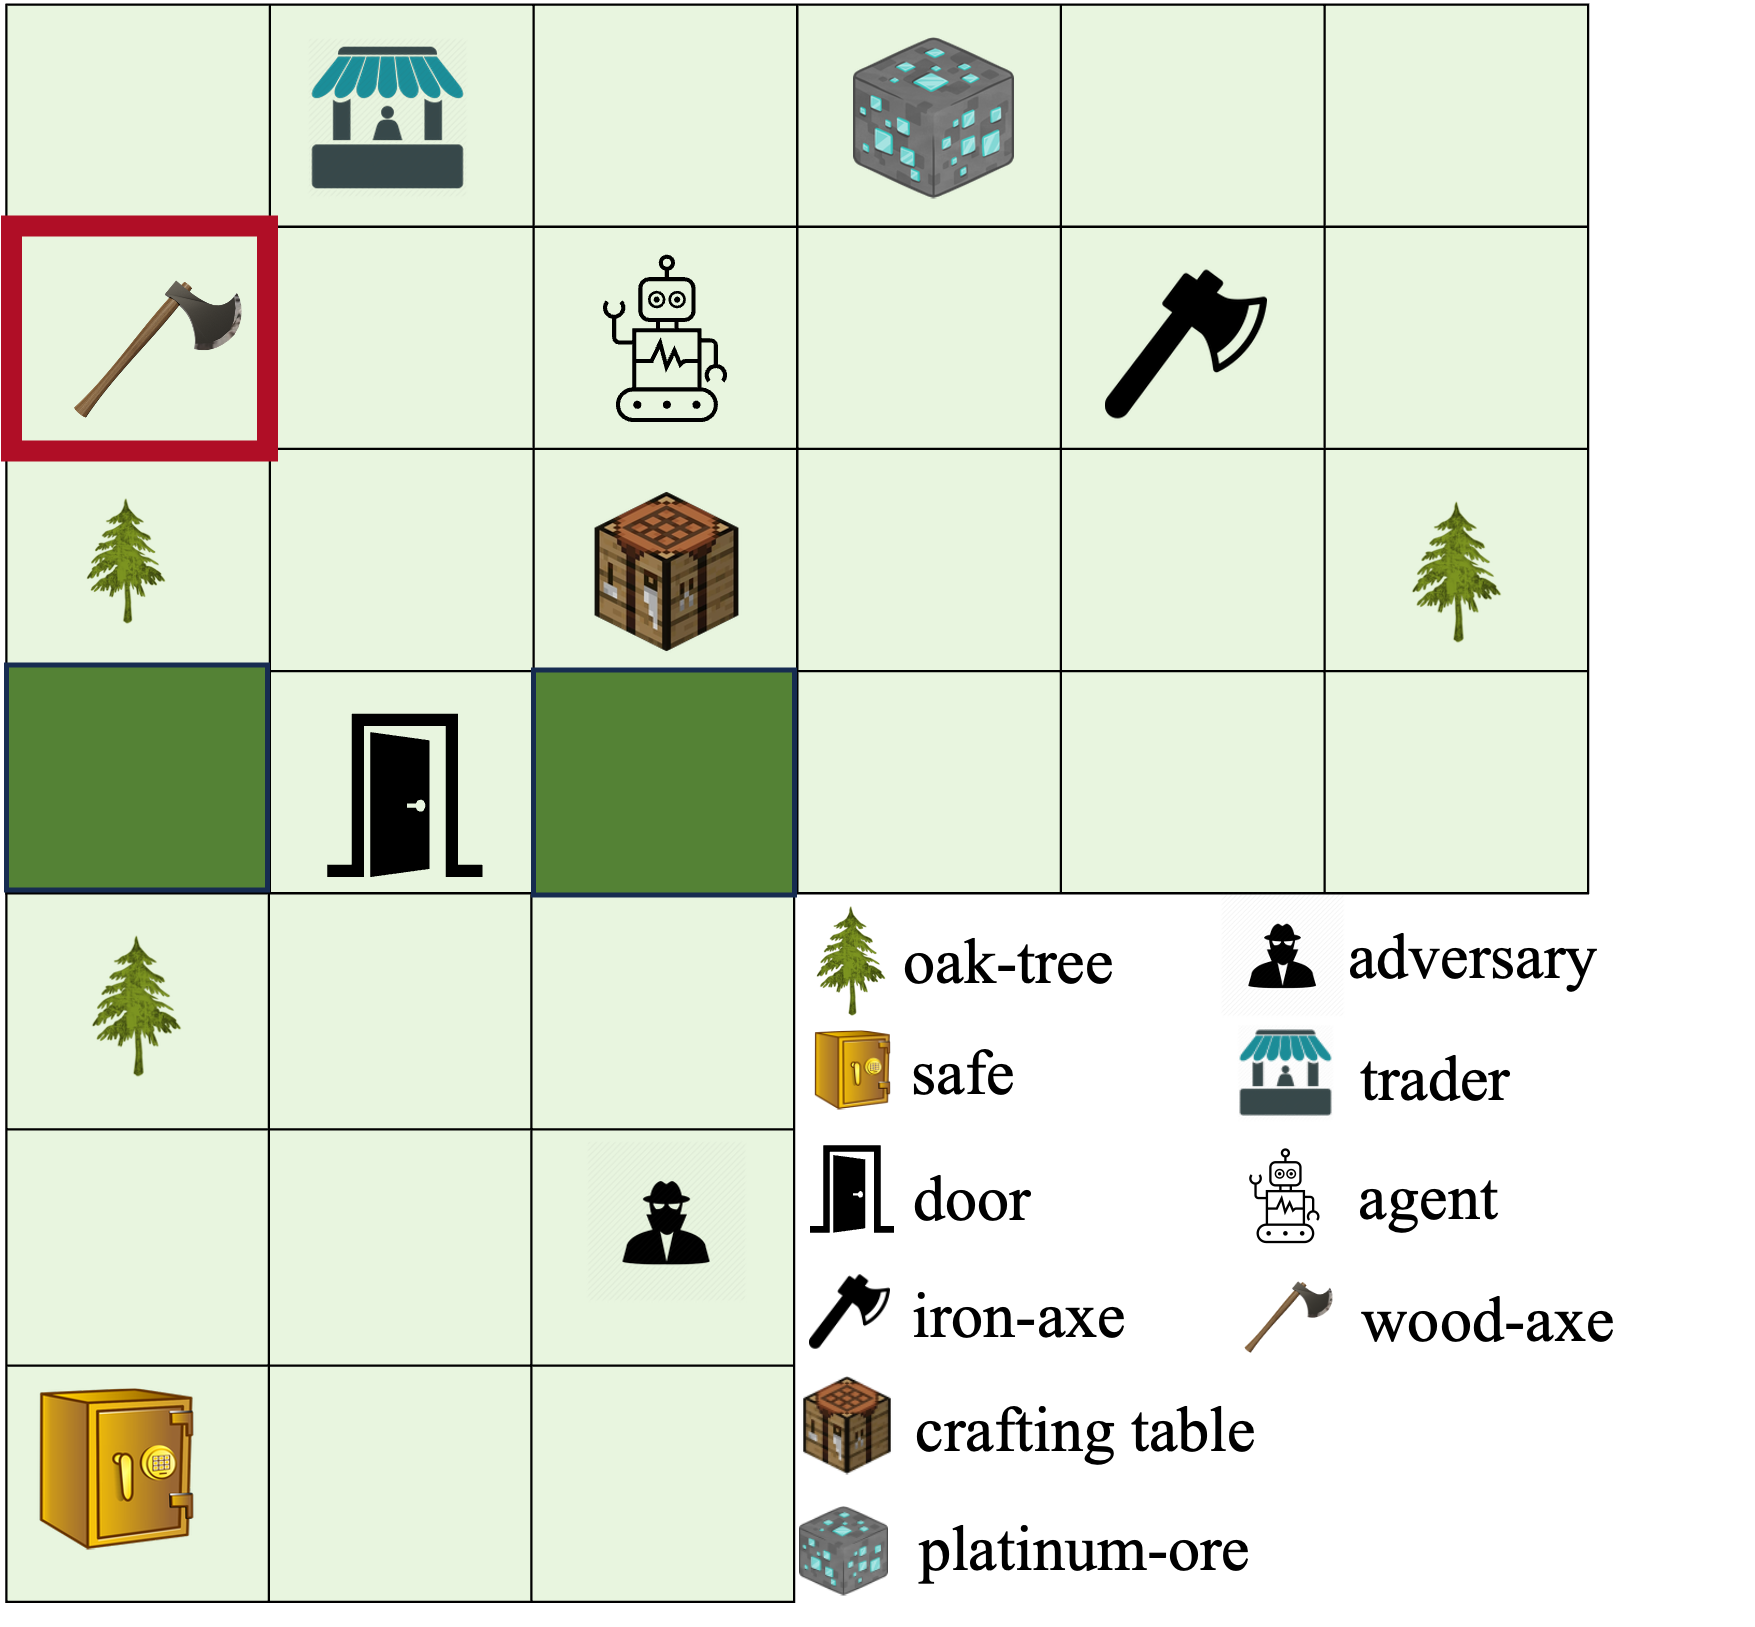
\includegraphics[width=0.6\textwidth]{figures/chapter2/Picture1_with_novelty.png}
\caption[The crafting gridworld environment]{The crafting gridworld environment used as a running example throughout this dissertation. The agent (center) operates among objects such as trees, crafting tables, and ores. A novel actor---the supplier, highlighted in blue---has been introduced and may affect the agent's ability to complete its task. Adapted from \citet{goel2024neurosymbolic}.}
\label{fig:gridworld}
\end{figure}

\subsection{Environment States and Agent Representations}
\label{sec:state_representations}

% The distinction between what exists in the environment and what the agent can represent is central to the framework.
 An environment state $e \in \EnvStates$ specifies the complete configuration of the world at a given time, including all objects, their properties, spatial arrangements, and dynamic relationships. The agent, however, does not operate over environment states directly. Instead, it constructs representations of the world using its available representational resources.

At the symbolic level, the agent uses a formal language $\Language$, consisting of predicates, variables, constants, and possibly functions, to describe aspects of the environment. A symbolic state description $\SymState \in \SymStates$ is a partial description of an environment state in this language. In planning domains, this description can be instantiated as a set of fluents $\Fluents$---state variables whose values may change over time---or as a set of grounded predicates that are used by the planner. When unlisted predicates are treated as false, this is a closed-world convention of the planning representation rather than a claim that the agent has complete knowledge of the environment.

At the subsymbolic level, the agent may represent the environment through continuous state vectors $s \in \States$, which may include raw sensory observations (e.g., images, Virtual LiDAR representations), learned feature representations, or structured numerical descriptions of the environment. These representations are typically used for perception and low-level control, and may be learned from data rather than explicitly defined. The agent's knowledge repository $\KnowledgeRepo$ contains the symbolic and subsymbolic representations that it uses to reason about the world and select actions. The inference mechanism $\vdash$ operates over these representations to generate plans, predict outcomes, and select actions. The agent's sensors and effectors mediate the mapping between the environment and its internal representations, but this mapping is not necessarily complete or accurate.

% An important consequence of this framework is that the mapping between environment states and agent representations is not one-to-one. Multiple environment states may be indistinguishable under the agent's current representational capacity, and a single environment state may be represented differently at different levels of abstraction. This gap between environment states and agent representations creates the space in which novelty can arise: aspects of the environment may exist, affect task performance, and yet not be derivable or representable within the agent's current knowledge repository.